\section{Architecture Overview}
The overall system architecture is depicted by Figure \ref{architecture_overview}.

To begin with, the whole system mainly operates within the user Local Area Network. A wireless router is the central point of the entire infrastructure because all the involved devices are connected to it via wireless communication.

The Raspberry Pi board is the backbone of the back-end processing activities. It is in charge of running Node-RED and acting as MQTT broker. It collects information that are sent out by several WiFi-capable modules taking advantage of the publish/subscribe MQTT connectivity protocol. Each module is provided with sensors that gather information about the surrounding environment.

ESP-12E and ESP-32 are the Wi-Fi boards that have been chosen to design the infrastructure. There exists a great variety of sensors that can be hooked up to these ESP modules and ease of programming via Arduino IDE makes them an appropriate choice too. Moreover, they offer full TCP/IP stack support.
Each board does not only publish data, but can also subscribe to a specific topic and receive remote commands to control actuators, such as relays.

The end user is able to visualize a user-friendly, web-accessible dashboard directly from his/her own devices, which must be in the same network of the other system components, in case port forwarding is disabled. The interface is provided by Node-RED development tool. Furthermore, data are forwarded to ThingSpeak by the Raspberry board in order to log them in a remote database and to enable further analysis: ThingSpeak has integrated support from the numerical computing software MATLAB.

\begin{figure}[H]
	\begin{center}
		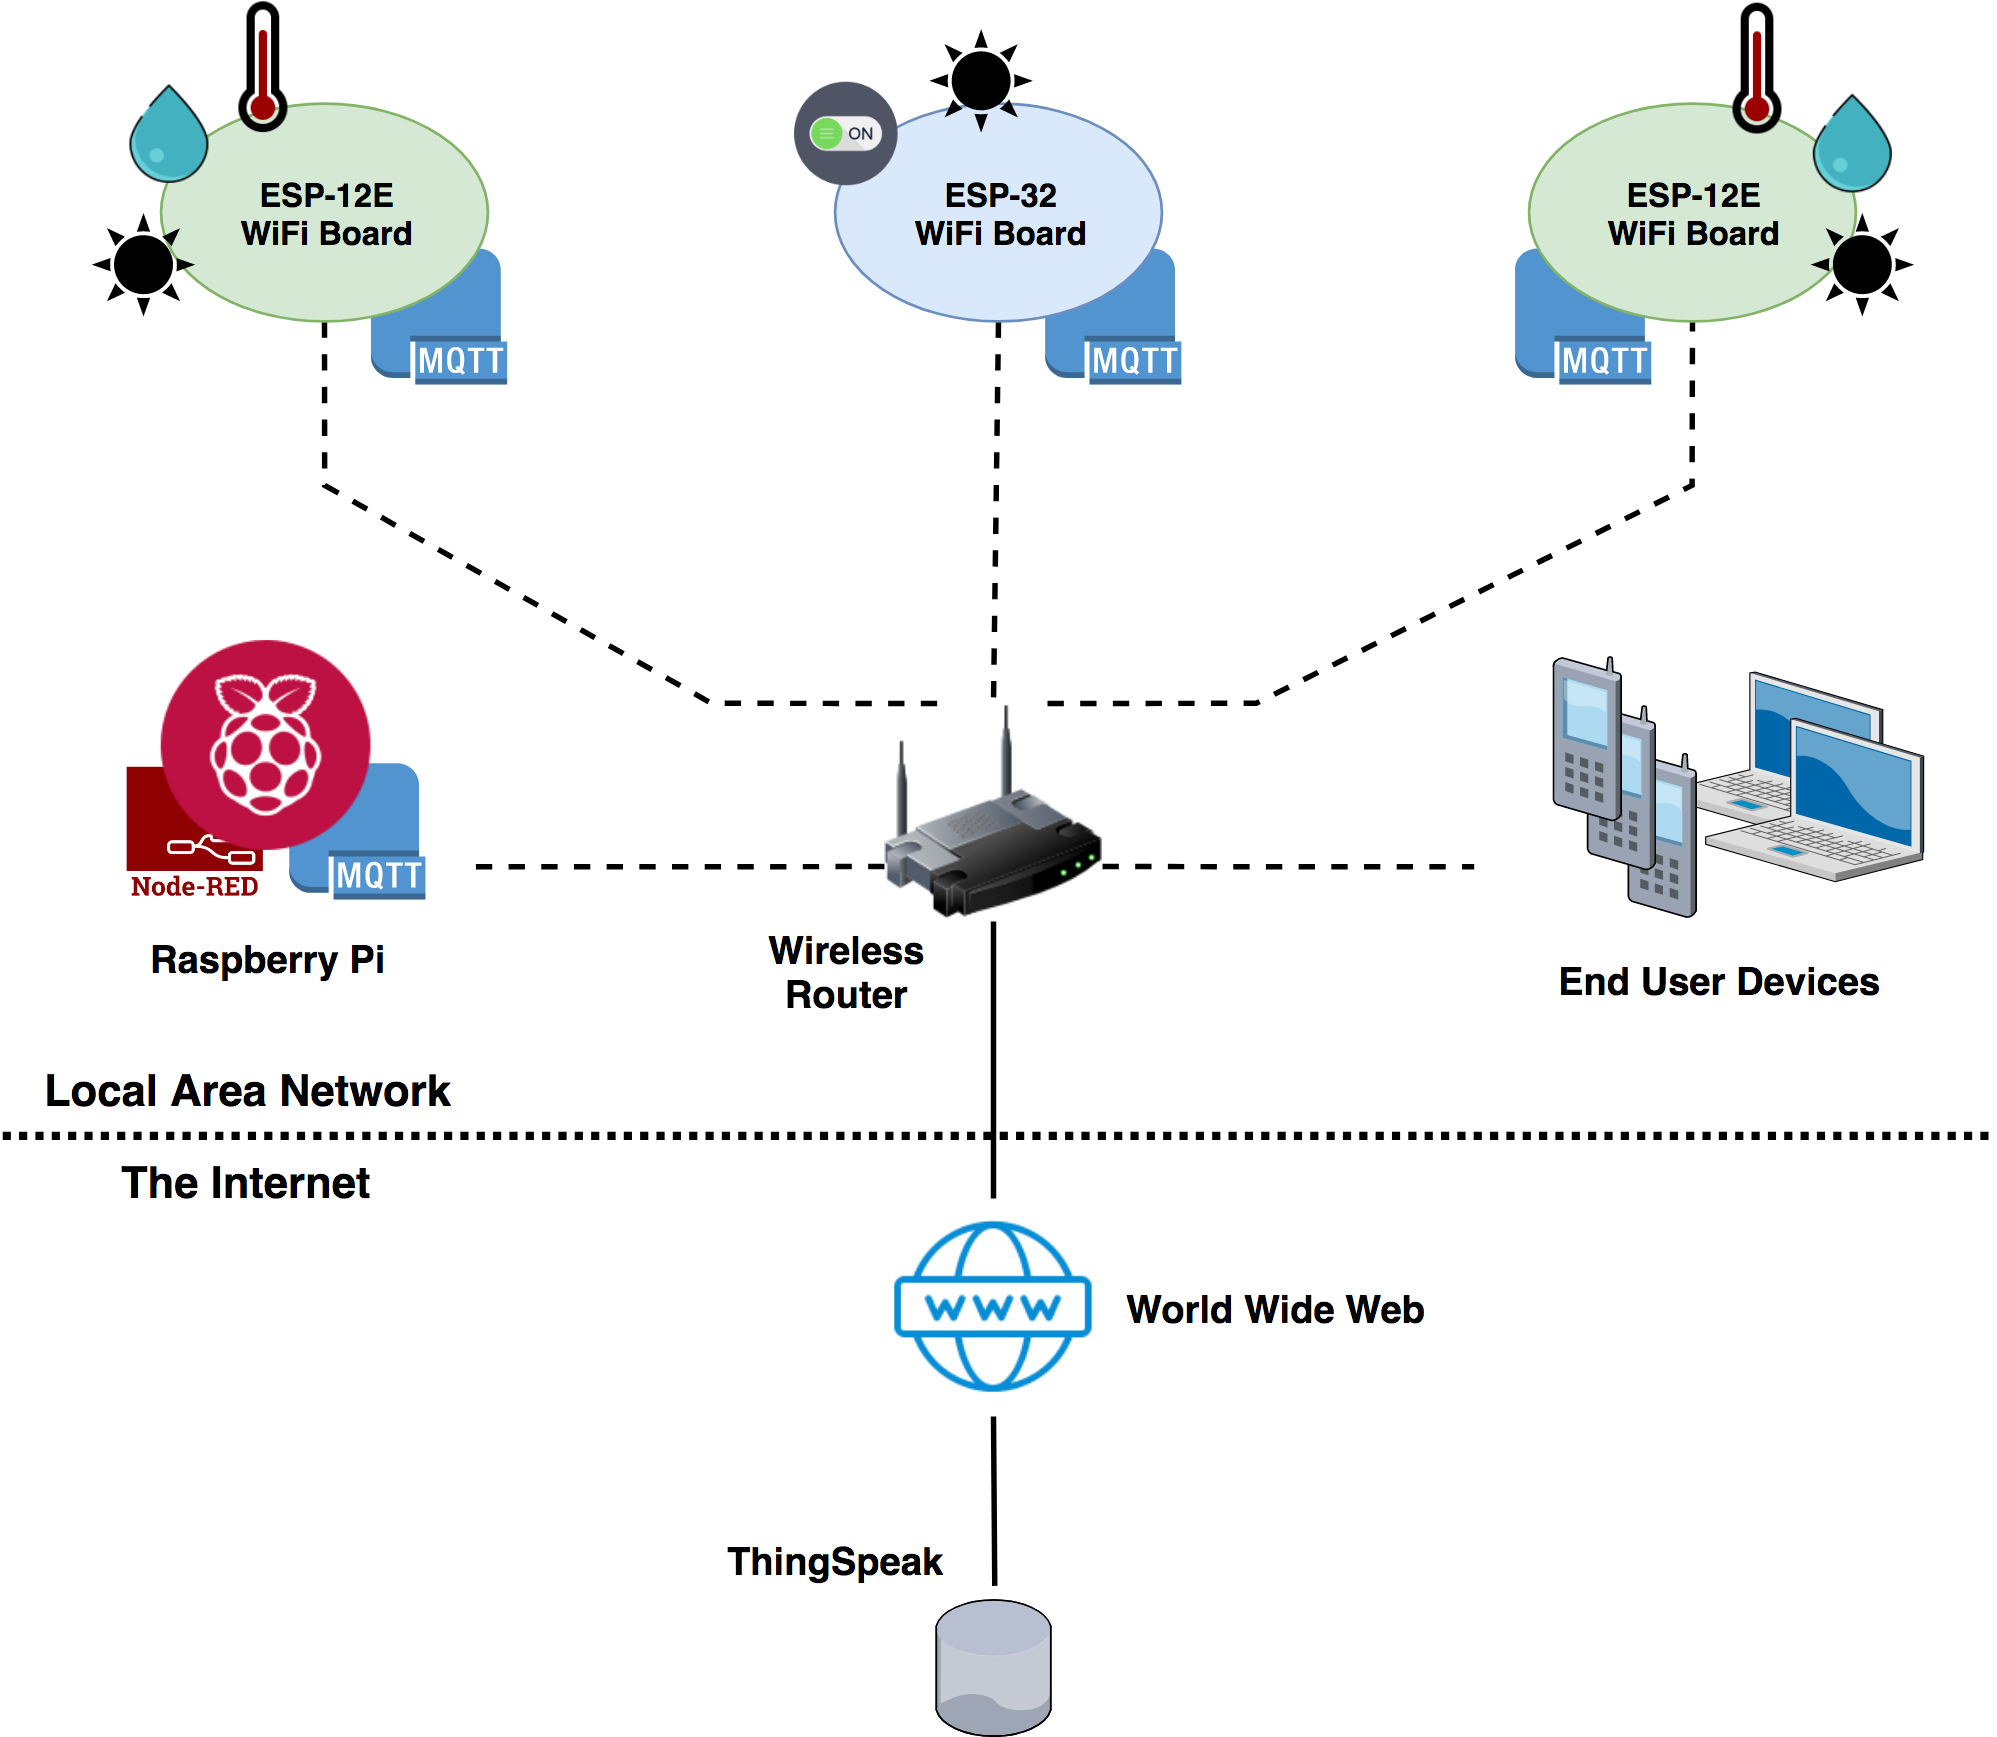
\includegraphics[width=\textwidth]{./pictures/architecture_overview.png}
		\caption{System architecture overview. Dashed lines represent wireless communication, solid lines stand for wired connections.}
		\label{architecture_overview}
	\end{center}
\end{figure}

\section{Configuring the RPi}
% suggerimento RPi 3
% indirizzo IP statico e connesione SSH per controllo remoto

\subsection{Mosquitto}
% Cos'è e cosa serve, MQTT in breve
% Installazione
% Configurazione credenziali
\subsection{Node-RED}
% Cos'è e cosa serve
% Sicurezza con credenziali
% Installazione dashboard
% Blocchi MQTT + credenziali
\section{Getting started with ESP boards}
% Schematici + commento codice
\section{Connecting to ThingSpeak}
% Cos'è e cosa serve
% Come ci colleghiamo al servizio?
% In breve come si usa